\pdfminorversion=7 % Set the PDF version to 1.7
\documentclass[czech,bachelor]{../../shared/diploma}

\usepackage{../../shared/additionallst} % Additional diploma thesis listings
\usepackage[autostyle=true,czech=quotes]{csquotes} % korektni sazba uvozovek, podpora pro balik biblatex
\usepackage[backend=biber, style=iso-numeric, alldates=iso]{biblatex} % bibliografie
\usepackage{dcolumn} % sloupce tabulky s ciselnymi hodnotami
\usepackage{subfig} % makra pro "podobrazky" a "podtabulky"
\usepackage{float} % lepsi umistovani obrazku (H)
\usepackage{bookmark} % Required for generating PDF bookmarks
\usepackage{subcaption}
\usepackage{hyperref}
\usepackage{tikz}
\usepackage{amsmath}

\renewcommand{\lstlistingname}{Zdrojový Kód} % Set your own caption name for listings

\newenvironment{plantuml}[1]{\VerbatimOut{#1.puml}}{\endVerbatimOut}
\newcommand{\processDiagram}[4]{%
    \IfFileExists{../../mik0486/target/puml/#2.pdf}{%
        \ifnum\pdfstrcmp{\pdffilemoddate{../../mik0486/target/puml/#2.pdf}}{\pdffilemoddate{#1.puml}}<0
            \immediate\write18{java -jar ../../shared/libs/plantuml-1.2024.3.jar -o ../../../mik0486/target/puml -tsvg #1.puml}
            \immediate\write18{inkscape ../../mik0486/target/puml/#2.svg --export-area-drawing --export-filename=../../mik0486/target/puml/#2.pdf}
        \fi
    } {%
        \immediate\write18{java -jar ../../shared/libs/plantuml-1.2024.3.jar -o ../../../mik0486/target/puml -tsvg #1.puml}
        \immediate\write18{inkscape ../../mik0486/target/puml/#2.svg --export-area-drawing --export-filename=../../mik0486/target/puml/#2.pdf}
    }

    \begin{figure}[H]
        \centering
        \includegraphics[width=#3]{../../mik0486/target/puml/#2}
        \caption{#4}\label{fig:#2}
    \end{figure}
}

% Pozadovane vstupy pro generovani titulnich stran.
\ThesisAuthor{Pavel Mikula}
\ThesisSupervisor{Ing. Radoslav Fasuga, Ph.D.}
\CzechThesisTitle{Tvorba administrativního rozhraní výpravné evoluční hry}
\EnglishThesisTitle{Creation of the Administrative Interface for the Narrative Evolution Game}
\SubmissionYear{2024}

\ThesisAssignmentFileName{../specification.pdf}

\CzechAbstract{
    Tato bakalářská práce se zabývá tvorbou administrativního rozhraní pro správu obsahu výpravné evoluční hry, které umožňuje kompletní operace nad objekty jako jsou postavy, předměty, lokace, události a další. Pro vytvoření administrativního rozhraní je prvně provedena analýza existujících řešení, návrh a následná implementace. Finálním produktem práce je funkční prototyp administrativní rozhraní, který umožňuje kompletní správu obsahu pomocí napojení na webové API, jež poskytuje data přímým přístupem k databázi.
}
\CzechKeywords{administrativní rozhraní, výpravně evoluční hra, správa obsahu hry, vykreslování, interaktivní editor}

\EnglishAbstract{
    This bachelor thesis focuses on the creation of an administrative interface for managing content in an elaborate evolutionary game, enabling complete operations over objects such as characters, items, locations, events, and more. Initially, an analysis of existing solutions is conducted, followed by the design and subsequent implementation. The final product of the thesis is a functional prototype of the administrative interface that allows complete content management through integration with a web API, which provides data via direct database access.
}
\EnglishKeywords{administrative interface, expansive evolutionary game, game content management, rendering, interactive editor}

\AddAcronym{AJAX}{Asynchronous JavaScript And XML}% {Asynchronní JavaScript A XML}
\AddAcronym{API}{Application Programming Interface}% {Rozhraní Pro Programování Aplikací}
\AddAcronym{CLI}{Command Line Interface}% {Příkazový Řádek}
\AddAcronym{CRUD}{Create, Read, Update, Delete}% {Vytvořit, Přečíst, Aktualizovat, Smazat}
\AddAcronym{CSRF}{Cross-Site Request Forgery}% {Mezisíťový Podvod}
\AddAcronym{CSS}{Cascading Style Sheets}% {Kaskádové Styly}
\AddAcronym{CSR}{Client-Side Rendering}% {Vykreslování Na Straně Klienta}
\AddAcronym{DOM}{Document Object Model}% {Dokumentový Objektový Model}
\AddAcronym{DTL}{Django Template Language}% {Django Šablonovací Jazyk}
\AddAcronym{Git}{Global Information Tracker}% {Globální Informační Sledovač}
\AddAcronym{GUI}{Graphical User Interface}% {Grafické Uživatelské Rozhraní}
\AddAcronym{HTML}{HyperText Markup Language}% {HyperTextový Značkovací Jazyk}
\AddAcronym{HTTPS}{HyperText Transfer Protocol Secure}% {Bezpečný Přenos Hypertextu}
\AddAcronym{MVC}{Model-View-Controller}% {Model-Pohled-Kontrolér}
\AddAcronym{MVT}{Model-View-Template}% {Model-Pohled-Šablona}
\AddAcronym{ORM}{Object-Relational Mapping}% {Objektově-Relační Mapování}
\AddAcronym{SEO}{Search Engine Optimization}% {Optimalizace Pro Vyhledávače}
\AddAcronym{SMS}{Short Message Service}% {Služba Krátkých Zpráv}
\AddAcronym{SPA}{Single Page Application}% {Aplikace Na Jedné Stránce}
\AddAcronym{SQL}{Structured Query Language}% {Strukturovaný Dotazovací Jazyk}
\AddAcronym{SSR}{Server-Side Rendering}% {Vykreslování Na Straně Serveru}
\AddAcronym{UI}{User Interface}% {Uživatelské Rozhraní}
\AddAcronym{UX}{User Experience}% {Uživatelská Zkušenost}
\AddAcronym{WebGL}{Web Graphics Library}% {Webová Grafická Knihovna}
\AddAcronym{WYSIWYG}{What You See Is What You Get}% {Co Vidíš, To Dostaneš}
\AddAcronym{XSS}{Cross-Site Scripting}% {Mezisíťové Skriptování}

\Acknowledgement{
    Rád bych na tomto místě poděkoval vedoucímu práce Ing. Radoslavu Fasugovi, Ph.D. za jeho cenné rady, trpělivost a ochotu věnovat mi svůj čas. Dále bych chtěl poděkovat svým kolegům Martinu Korotwitschkovi, Barboře Kovalské a Miroslavu Osobovi za jejich asistenci při vývoji.
}

% Novy druh tabulkoveho sloupce, ve kterem jsou cisla zarovnana podle desetinne carky
\newcolumntype{d}[1]{D{,}{,}{\#1}}

\addbibresource{resources/sauce.bib}

% Zacatek dokumentu
\begin{document}

% Titulni strany
\MakeTitlePages

% Obrazky
\listoffigures
\clearpage

% Tabulky
\listoftables
\clearpage

% Úvod
\chapter{Úvod}
\label{ch:introduction}


\endinput

% Kapitoly
\chapter{Teorie a analýza}
\label{ch:theory_and_analysis}
V této kapitole se práce věnuje teorii a analýze rozhraní, včetně jejich klíčových prvků, které jsou zásadní pro pochopení základních principů efektivního designu jak uživatelských, tak i administrativních rozhraní. Dále je zaměřena na analýzu populárních deskových her, které si v současné době získaly velkou popularitu a zájem hráčů. V závěru kapitoly jsou popsány na administrativní prvky a značky, které jsou zásadní pro správu obsahu aplikace.

\section{Teorie UI/GUI}
\label{sec:ui-gui-theory}
Uživatelské rozhraní z anglického jazyka \textit{\textquote{User Interface}} (UI) a grafické uživatelské rozhraní \textit{\textquote{Graphical User Interface}} (GUI) jsou termíny používány v kontextu digitálních aplikací, kde tyto prvky umožňují uživatelům interagovat se softwarem aplikace pomocí rozhraní. Zatímco UI zahrnuje jakoukoliv formu uživatelského rozhraní, GUI se specificky zaměřuje na vizuální aspekty rozhraní, jako jsou okna, ikony, tlačítka a další grafické elementy.

Základem dobrého UI je především jeho intuitivita, jednoduchost a přehlednost, což jednoduše znamená, že by uživatel měl být schopen jednoduše pochopit jak s aplikačním rozhraním pracovat, aniž by musel procházet složitějším procesem učení.

\subsection*{Klíčové prvky UI/GUI}
\label{subsec:ui-gui-theory-key-elements}
\begin{itemize}
    \item \textbf{Rozložení} -- Efektivní rozložení usnadňuje uživatelskou orientací, uživatelé pak snadnější naleznou potřebné funkce nebo informace.
    \item \textbf{Prvky ovládání} -- Tlačítka, menu, přepínače a další administrativní prvky by měly být v ideálním případě jasně označené a snadno dostupné.
    \item \textbf{Typografie a barevnost} -- Výběr písma a jeho barevné schéma hraje významnou roli v čitelnosti a celkovém vnímání. V dnešní době se stránky hodně zaměřují na tmavá přepínatelná pozadí známá jako \textit{Dark Mode} a \textit{Light Mode}.
    \item \textbf{Interaktivita} -- Při podání vstupu do aplikace by uživatelé měli dostat okamžitou zpětnou vazbu, čímž dostávají informaci, že jejich akce byla zpracována nebo se aktuálně zpracovává. Často je probíhající akce vyobrazena určitým opakujícími se animacemi například tak točící se kolečko známé jako \textit{loading spinner}.
    \item \textbf{Přizpůsobivost} -- Možnost přizpůsobit si uživatelské rozhraní zvyšuje celkovou přívětivost, v rozhraních tak většinou nalezneme možnost změnit jazyk, barvy nebo pozice jednotlivých oken. Tyto změny se většinou uchovávají pouze v uložišti prohlížeče a nejsou nijak sdílený mezi zařízeními.
\end{itemize}

\subsection*{Principy dobrého UI designu}
\label{subsec:ui-gui-theore-basic-use-case}
\begin{itemize}
    \item \textbf{Konzistence} -- Při provádění stejné akce, by uživatel měl pokaždé dostat stejnou odpověď.
    \item \textbf{Jednoduchost} -- UI by mělo mít minimalistický design, který je hlavně zaměřen na důležité funkce.
    \item \textbf{Přívětivost} -- Uživatel by měl být schopen, okamžitě pochopit rozložení UI bez nutnosti se ho učit.
    \item \textbf{Dostupnost} -- UI by mělo být dostupné pro všechny uživatele, bez ohledu na jejich schopnosti.
    \item \textbf{Zabezpečení} -- UI by mělo být zabezpečené a chránit uživatele před různými útoky.
    \item \textbf{Responzivita} -- UI by mělo být responzivní a přizpůsobit se různým zařízením.
    \item \textbf{Zpětná vazba} -- Uživatel by měl být informován o každé akci, kterou provedl.
\end{itemize}

\subsection{Počátek vzniku rozhraní}
\label{subsec:ui-gui-theory-beginning}
Vznik rozhraní lze vysledovat až k raným počátkům počítačů, kde se interakce mezi uživatelem a rozhraním prováděla pomocí děrných štítků a přepínačů. Postupem času s vývojem technologií vzniklo rozhraní terminálové z anglického jazyka \textit{\textquote{Command Line Interface}} (CLI), které obsahovalo základní textový vstup z klávesnice a následného výstupu umístěného na displej. Toto rozhraní se stalo standardem pro každý novodobý počítač a používá se do dnešních let. Zlomovým momentem se poté stal příchod grafického rozhraní z angl. \textit{\textquote{Graphical User Interface}} (GUI), které znamenalo revoluci v přístupu k interakci uživatele s počítačem. Tato evoluce přinesla nové možnosti pro uživatele, jak přímo komunikovat s počítačem díky grafickým prvkům jako jsou okna, ikony, menu za pomocí pohybu myši po obrazovce.

Pro nás se grafická reprezentace v počítači stala již nedílnou součástí našeho života a v dnešní době se s ní setkáváme již na každém kroku, ať se jedná o mobilní aplikace, počítačové aplikace nebo prosté webové stránky.

Pro vývoj webových aplikací se většinou používají technologie spojené pomocí jazyku JavaScript. V minulých letech, zde ale existoval software se jménem \textit{Adobe Flash Player}, který umožňoval vytvářet interaktivní multimediální obsah, který se mnohdy využíval na vývoj různých webových aplikací, ať se jednalo o různé hry, prezentace nebo třeba aplikaci fotogalerie. Bohužel tento software byl koncem roku 2020 ukončen a nahrazen modernějšími a bezpečnějšími technologiemi, které zároveň stály za jeho úpadkem. Mezi tyto technologie se řadí HTML5, WebGL nebo WebAssembly. \cite{adobeFlashPlayer-eol}

\subsection{Problematika vývoje}
\label{subsec:ui-gui-theory-problems}
Problematika vývoje rozhraní se týká komplexního procesu, který zahrnuje několik oblastí, nad kterými je potřeba se předem zamyslet a následně je implementovat. Většinou při zanedbaní správné implementace těchto sekcí, lze v budoucnu rychle dosáhnout problémů, kde jejich řešení může mít výrazný vliv na funkčnost aplikace. Mezi tyto oblasti spadá například:

\begin{description}
    \item \textbf{Uživatelský vstup}, který reprezentuje, jakým způsobem bude uživatel nebo administrátor aplikaci podávat vstup. Tedy jestli se jedná o textový vstup, vstup ovládáním myši nebo dotykovým displejem. Dle tohoto kritéria se poté volí vhodný způsob zpracování vstupu.
    \item \textbf{Vykreslování}, které se většinou rozděluje na potřeby uživatelské a administrativní částí. Kde uživatelská se zaměřuje více na design a přívětivost pro uživatele, zatímco administrativní se zaměřuje na efektivitu a snadnou správu obsahu. Tento rozdíl můžeme jednoduše vidět na tom, že administrativní rozhraní využívá plný potenciál obrazovky, zatímco uživatelské se snaží dbát na přehlednost a jednoduchost.
    \item \textbf{Responzivní design} určuje, jak se jednotlivé prvky na obrazovce zachovají při změně velikosti okna nebo zařízení. Aplikace by v ideálním případě po změně velikosti neměla ztratit na přehlednosti nebo jakkoliv poškodit uživatelskou zkušenost. U mobilních verzí aplikací se objevují separátní odkazy na nativní rozhraní, které se nachází pod subdoménou s název \textquote{m} tedy například \textit{https://m.tts-game.fun}\footnote{Nejedná se o funkční odkaz ale pouhou referenci.}. Řešení responzivního designu dále bude pokračovat v samostatné Podkapitole~\ref{subsec:ui-gui-theory-responsive-design}.
    \item \textbf{Uživatelská zkušenost} z anglického jazyka \textit{\textquote{User Experience}} (UX) se soustředí na to, jak uživatelé vnímají a jak se cítí při používání aplikace. Tedy jak je aplikace přívětivá, snadno ovladatelná a zda splňuje očekávání uživatele.
    \item \textbf{Bezpečnost} je důležitým aspektem, který se zaobírá zpracováním uživatelských dat, které v mnoha případech obsahují citlivé informace. Při nesprávném zpracování těchto dat může dojít k úniku dat nebo jejich zneužití. Jako řešení se používají různé techniky, jako je například šifrování, ověřování uživatele nebo zabezpečení připojení.
\end{description}

\subsection{Responzivní design}
\label{subsec:ui-gui-theory-responsive-design}
Responzivní design se stal již skoro povinným standardem pro všechny webové stránky a aplikace. Tento přístup se zaměřuje na webové prvky tak, aby při jejich zobrazení na různých zařízeních s rozdílnou velikosti obrazovky nebo orientace byly pořád stejně přehledné a plně funkční. Této funkčnosti se dosahuje pomocí kaskádových stylů (CSS), které tuto funkcionalitu umožňují pomocí tzv. \textit{\textquote{media queries}}. Tyto dotazy umožňují nastavovat styly podle předem daných kritérii, jako například šířka okna, výška okna, typ zařízení nebo jeho orientace.

Jedním z průkopníků responzivního designu se stal \textit{Bootstrap}, open-source framework pro vývoj front-end webových aplikací, který nabízí soubor knihoven a předem vytvořených šablon stylů, díky kterým je možné za použití pár elementů dosáhnout rychlého a plně responzivního designu aplikace. Tento framework je v současné době jedním z nejpoužívanějších z důvodu jeho lehkého nasazení, široké podpory a velké kompatibility. Využití potenciálu tohoto frameworku si blíže popíšeme v Kapitole~\ref{subsec:dev-technology-bootstrap}.

\lstinputlisting[language=CSS, caption={Příklad použití media query v css.}, label={lst:media-query-example}]{sourceCodes/MediaQueryExample.css}

Ve stručném vysvětlení Zdrojového kódu~\ref{lst:media-query-example} můžeme vidět, že se jedná o základní CSS kód, který nastavuje barvu pozadí stránky na světle šedou. Obsahuje ale také média dotaz na řádku 6, který se ptá na velikost obrazovky, kde v případě, že je šířka obrazovky menší než 600px, změní barvu pozadí na světle modrou.

\begin{figure}[H]
    \centering
    \includegraphics[width=1.0\textwidth]{figures/responsiveDesign}
    \caption{Ukázka responzivního designu mezi zařízeními. \cite{responsive_design}}
    \label{fig:responsive-design-example}
\end{figure}

\section{Analýza populárních deskových her}
\label{sec:popular-board-games-analysis}
Deskových her je v dnešní době na trhu velké množství, kdy se každým novým rokem se snaží noví nebo i stálí autoři proniknout ven s novými nápady nebo koncepty. Deskové hry lze rozdělit na několik herních žánrů, jako jsou například hry strategické, kooperativní, party, rodinné nebo třeba karetní. Velká většina z těchto her se zaměřuje na její plný průběh na půdě hracího stolu, existují zde ale i hry, které do tohoto průběhu zapojují i externí zařízení, jako jsou speciální zařízení, mobilní telefony nebo laptopy. Tyhle hry se nazývají hry hybridní, kde jejich bližší definici popíšu v následující sekci.

\subsection*{Hybridní hry}
\label{subsec:popular-board-games-analysis-hybrid-games}
Jak již bylo zmíněno o sekci výše, hybridní hry jsou hry takové, které kombinují jednotlivé funkční prvky z her fyzických nebo digitálních. Jednoduše se dá říci, že hybridní hra je hra taková, která má jakékoliv napojení na technologii. Mezi hry hybridní patří například populární hra \textit{Monopoly}, která používá speciální bankovní zařízení používané pro správu financí nebo hra \textit{XCOM: The Board Game}, která využívá mobilní aplikaci pro správu herního průběhu.

\subsection{Populární deskové hry}
\label{subsec:popular-board-games-analysis-popular-games}
Populárních deskových her je na světě velké množství, Z toho důvodu jsem pro tuto analýzu pouze hry, které mi jsou nejbližší a již jsem měl možnost si je zahrát. Díky této zkušenosti můžu lépe popsat možnosti a prvky, které tyto hry obsahují. Mezi tyto stolní hry patří například \textit{Carcassonne}, \textit{Bang!}, \textit{Codenames} nebo \textit{Gloomhaven}. Bohužel během analýzy se mi nepodařilo nalézt žádnou z her, která by měla k dispozici veřejné administrativní rozhraní. Z logického pohledu je totiž administrativní rozhraní limitováno pouze pro administrátory dané hry. V následujících podkapitolách jsou popsány především hry, které obsahují alespoň jejich online verze nebo příslušné nástroje pro rozšíření herního zážitku.

\subsubsection{Carcassonne}
\label{subsubsec:popular-board-games-analysis-carcassonne}
Carcassonne je desková stolní hra, vydaná v roce 2000 autorem \textit{Klaus-Jürgen Wrede}. Hra je založena na jednoduchém principu losování a skládání herního pole, které se skládá z dlaždic obsahujících různé herní prvky. Hra je určena pro 2 až 5 hráčů, kde reálný počet hráčů závisí na velikosti skupinek hráčů nebo počtu rozšíření. Hra je velmi oblíbená převážně pro svůj jednoduchý herní styl, který je tak zábavný pro všechny věkové kategorie.

\subsubsection*{Rozšíření}
\label{subsubsec:popular-board-games-analysis-carcassonne-expansions}
Carcassonne jako základní hra sama o sobě disponuje obstojnou délkou hraní okolo 45 minut až hodiny a půl. Existuje zde ale mnoho rozšíření, které se rozdělují na obyčejné a mini a tento herní čas dokáží hravě prodloužit. Mezi nejznámější rozšíření patří například \textit{Carcassonne: Hostince a katedrály} nebo \textit{Carcassonne: Kupci a stavitelé}. Každé z rozšíření se pohybuje kolem 330 Kč, kde základní hra stojí kolem 600 Kč.

\subsubsection*{Online verze}
Hra se stala rychle populární a tak se brzy objevila i její online varianta ať se jedná o hru ve webovém prohlížeči, mobilní aplikaci nebo na herní platformě \textit{Steam}\footnote{Steam je herní platforma vyvinutá společností Valve, která slouží pro distribuci digitálních her, software a dalších služeb.}. Online verze hry umožňuje hráčům hrát s ostatními hráči po celém světě, kde mezi sebou hráči můžou soupeřit v turnajích nebo v žebříčcích.

\subsubsection{Bang!}
\label{subsubsec:popular-board-games-analysis-bang}
Bang je karetní hra, vydaná v roce 2002 autorem \textit{Emiliano Sciarra}. Hra je založena do tématiky westernového světa, kde hráči hrají postavy z divokého západu jako je šerif, zástupce šerifa, bandité nebo odpadlíci. Hra je určena pro 4 až 7 hráčů a jejím cílem je vždy splnit cíl dané role. Hráč si vždy na začátku vylosuje 2 postavy a příslušnou roli. Poté si vybere jednu z postav a hra začíná. Hra je velmi populární z důvodu nenáročného herního stylu na okolní hráče.

\subsubsection*{Rozšíření}
\label{subsubsec:popular-board-games-analysis-bang-expansions}
Bang! stejně jako Carcassonne obsahuje několik možných rozšíření, které do hry dodávají nové prvky a postavy. Její nejznámější rozšíření jsou například \textit{Bang! Zlatá horečka} nebo \textit{Bang! Velká vlaková loupež} a další. Hra opět obsahuje několik minirozšíření, které do hry dodávají pouze nové postavy nebo karty, oproti velkým rozšířením, které do hry dodávají herní předměty. Každé z rozšíření se tak pohybuje kolem 350 Kč a základní verze hry stojí 400 Kč.

\subsubsection*{Online verze}
Stejně, jako hru Carcassone, lze i tuto hru hrát kompletně online. Hra Bang! se více zaměřuje na svoji kompetitivní stránku, kde hráči často hrají proti sobě na body. Čím více bodů hráč má, tím lepší protivníky následně proti sobě získává. Hra obsahuje i herní mód, kde hráči mohou hrát proti počítači, kde mohou trénovat své dovednosti nebo se připravit na online hraní. Při navštívení komunitní stránky hráč může po registraci nebo přihlášení vyhledat volnou místnost kde bude automaticky přiřazen.

\subsubsection{Codenames (Krycí jména)}
\label{subsubsec:popular-board-games-analysis-codenames}
Krycí jména z anglické verze \textit{Codenames} se dá považovat za karetní hru s drobnými prvky z her stolních. Hra byla vydaná v roce 2015 autorem \textit{Vlaada Chvátil}. A přináší další hru z žánru kooperativně kompetetivních, kde jsou hráči rozdělení do 2 týmu a každý tým má svého hlavního špiona. Hra je určena pro 4 až 8 hráčů a jejím cílem je správně uhádnout všechny karty na herním poli. Jednoduchost hry vypovídá i z faktu, že si lze všechny důležité komponenty vyrobit doma za pomocí tiskárny.

\subsubsection*{Online verze}
\label{subsubsec:popular-board-games-analysis-codenames-online}
Oproti hře \textit{Bang!} a \textit{Carcassonne} hra Codenames má svoji originální online verzi dostupnou pod odkazem\footnote{https://codenames.game/} vytvořenou přímo autorem hry stolní. Tato verze hry oproti ostatním nedisponuje žádným kompetetivním žebříčkem, ale reprezentuje se jako online možnost zahrát si tuto hru s přáteli přes internet. Po otevření stránky hra nabízí možnost založit místnost, kde lze pomocí speciální odkazu pozvat do hry další hráče. Následně se hráči mohou rozřadit do týmů a následně začít hrát.

\subsubsection{Gloomhaven}
\label{subsubsec:popular-board-games-analysis-gloomhaven}
Gloomhaven je desková stolní hra, vydaná v roce 2017 autorem \textit{Isaac Childres}. Hra je založena na tématice a herním principu hry \textit{Dungeon and Dragons} a je dostupná pro 1 až 4 hráče. Princip hry je oproti ostatním násobně složitější a celá hra je náročna na strategii a taktiku. Pro hru je potřeba mít dostatečný čas a trpělivost, jelikož hra může trvat i několik hodin.

Hra se pyšní i svou velikosti herní krabice, která obsahuje více než 300 herních komponentů, které se skládají z karet, tokenů, figur a herních plánů. Hru je nutné hrát v dostatečně velké místnosti s adekvátním stolem na rozmístění všech komponentů.

\subsubsection*{Podpůrné nástroje}
\label{subsubsec:popular-board-games-analysis-gloomhaven-support-tools}
Kvůli celkové velikosti a ceně hry samotné, jenž se pohybuje okolo 3000 Kč, se vytvořila komunita, která se pokusila vytvořit několik podpůrných aplikací pro zlepšení a zjednodušení herního průběhu. Jednotlivé nástroje si trošku popíšeme v následujících podkapitolách.

\begin{description}
    \item \textbf{Gloomhaven Helper}\footnote{\href{https://en.esotericsoftware.com/gloomhaven-helper}{https://en.esotericsoftware.com/gloomhaven-helper}} je nativní aplikace, která podporuje kompletní přesun dění ze stolu na obrazovku. Díky čemuž hráči nemusí pořád přepočítávat životy, počty nepřátel nebo tahat útokové karty. \footnote{Aplikace již není dostupná z licenčních důvodu autora hry.}
    \item \textbf{Gloomhaven Full Stack V2}\footnote{\href{https://gloomhaven.smigiel.us/v2/}{https://gloomhaven.smigiel.us/v2/}} je pouze webová alternativa zrušeného gloomhaven helperu, která podobným způsobem dovoluje uživatelům zaznamenávat plný průběh dění ve webovém prostředí.
    \item \textbf{Gloomhaven Storyline}\footnote{\href{https://gloomhaven-storyline.com/}{https://gloomhaven-storyline.com/}} je další z možných aplikací, která se zaměřuje na zjednodušení herního průběhu. Aplikace obsahuje kompletní přehled o herním světě, postavách a úkolech.
\end{description}

\section{Administrativní prvky}
\label{sec:admin-elements}
Každé administrativní rozhraní se skládá z několika základních prvků, které umožňují uživatelům s administrativním oprávněním provádět specifické úkony nebo měnit kompletní nastavení aplikace. Mezi takové prvky patří například správa uživatelů, obsahu, nastavení, zobrazení statistik nebo přehled logů. V následujících podkapitolách se blíže zaměřím na tyto jednotlivé prvky.

\subsection{Správa uživatelů}
\label{subsec:admin-elements-user-management}
Správa uživatelů je nedílnou součástí každého sofistikovaného systému nebo aplikace, která umožňuje administrátorům ovlivňovat, kdo může přistupovat k jednotlivým částem systému. Tento prvek systému umožňuje nejen přidávat, odstraňovat nebo měnit uživatele, ale také udělovat jejich oprávnění, role nebo měnit nastavení. Mezi časté role patří například \textit{administrátor}, \textit{editor}, \textit{moderátor} nebo výchozí \textit{uživatel}. Každá role má přidělený seznam oprávnění, které určují co může uživatel dělat a co ne.

Tento přístup následně umožňuje vytvářet hierarchii uživatelů, kde administrátor má plný přístup ke všem funkcím aplikace, zatímco uživatel má pouze omezený přístup, čímž zvyšuje bezpečnost a efektivitu aplikace. Správa uživatelů obsahuje nástroje pro sledování aktivity uživatelů nebo jejich záznam provedených akcí. Na Obrázku~\ref{fig:user-management} můžeme vidět ukázku uložení uživatele v databázi.

\begin{figure}[H]
    \centering
    \includegraphics[width=0.7\textwidth]{diagrams/userManagement}
    \caption{Ukázka uložení uživatele v databázi. \cite{responsive_design}}
    \label{fig:user-management}
\end{figure}

\subsection{Správa obsahu}
\label{subsec:admin-elements-content-management}
Jako u správy uživatelů, správa obsahu z anglického jazyka \textit{\textquote{Content Management}} je dalším a hlavním pilířem administrativních rozhraní. Tento prvek umožňuje výše zmíněným rolím vytvářet, upravovat a odstraňovat obsah tak, že není nutné jakkoliv zasahovat do kódu aplikace nebo měnit čistá data ručně v databázi. Tento prvek je zásadní pro dynamické webové stránky, e-commerce platformy, blogy a další aplikace, které pravidelně mění svůj obsah nebo provádí jejich další vývoj.

Textová editace obsahu v aplikacích se provádí pomocí interaktivních editorů, které jsou součástí formulářů. Takové editory se nazývají WYSIWYG z anglického \textit{\textquote{What You See Is What You Get}}, tyto editory umožňují uživatelům editovat obsah, aniž by museli znát HTML nebo CSS. Tento způsob editace je velmi oblíbený pro svou jednoduchost a přehlednost, která umožňuje i méně zkušeným uživatelům editovat obsah bez jakýchkoliv problémů. Mezi tyto populární editory patří CKEditor\footnote[1]{\url{https://ckeditor.com/}}, TinyMC\footnote[2]{\url{https://www.tiny.cloud/}} nebo Quill\footnote[3]{\url{https://quilljs.com/}}.

\subsection{Nastavení}
\label{subsec:admin-elements-settings}
Sekce pro nastavení se nachází v každém administrativním rozhraní a umožňuje administrátorům přizpůsobovat aplikaci podle specifických potřeb a preferencí. To může zahrnovat širokou škálu možností začínající od změny barvy, jazyka, loga, až po pokročilé možnosti jako je změna způsobu zabezpečení, různé integrace aplikací třetích stran a časté upravování SEO nastavení, které zlepšuje viditelnost aplikace ve vyhledávačích.

\subsection{Statistiky}
\label{subsec:admin-elements-statistics}
Statistiky poskytují ucelený přehled o využití a výkonost aplikace. Kde se zaměřuje na analýzu návštěvnosti, sledování chování uživatelů nebo sledování výkonu aplikace. Tento prvek umožňuje administrátorům sledovat aktuální stav aplikace a provádět potřebné úpravy pro zlepšení výkonu nebo zvýšení návštěvnosti.
Tyto statistiky se většinou zobrazují v podobě grafů, tabulek nebo zpráv, které poskytují uživatelům přehledné informace o aktuálním stavu aplikace.

Nástroje pro sledování statistik se používají Google Analytics\footnote[4]{\url{https://analytics.google.com/}}, Matomo\footnote[5]{\url{https://matomo.org/}} nebo Yandex Metrica\footnote[6]{\url{https://metrica.yandex.com/}}. Při používání těchto nástrojů třetích stran je nutné dbát na zabezpečení a ochranu uživatelských dat, které tyto nástroje zpracovávají.

\subsection{Záznam akcí}
\label{subsec:admin-elements-logs}
Systém zaznamenávání známý jako \textit{Audit Log} je nezbytným nástrojem pro monitorování a diagnostiku problému v aplikaci. Umožňuje zaznaménávat události, jako jsou chyby, varování, informační zprávy nebo auditní záznamy o aktivitách uživatelů. Zpětné zobrazování záznamů pomáhá administrátorům rychle identifikovat a vyřešit problém dříve než dojde k jejich zvěřejnění nebo zneužití. Čímž zajišťují bezpečný a nepřetržitý průběh aplikace.

\section{Administrativní značky}
\label{sec:admin-tags}
Administrativními značkami se rozumí prvky HTML, které jsou specifické pro přijímání požadavků od uživatele nebo uživateli předávají informace. Mezi takové značky patří například formuláře, tlačítka, tabulky nebo grafy. Jednotlivé značky se v nižších sekcích pokusím blíže přiblížit.

\subsection*{Menu}
\label{subsec:admin-tags-menu}
Menu je zásadním navigačním prvkem v jakémkoliv rozhraní, umožňující uživatelům snadný přístup k rozdílným částem aplikace. Tento prvek se nachází v horní částí aplikace nebo v její levé části a obsahuje odkazy na podřadné stránky. Důležitá je efektivnost navržení menu, kde se klade důraz na uživatelskou přívětivost a rychlou orientaci. Při velkém a rozsáhlém stromu menu v opačném případě dochází k častému zmatení uživatele, který stránku opouští.

\subsection*{Formulář}
\label{subsec:admin-tags-form}
Formuláře jsou klíčové pro interakci s uživatelem, neboť umožňují aplikaci přijímat datový vstup od uživatelů. Častým výskytem formulářů v administrativních rozhraních jsou stránky určené pro přihlášení, registraci, zadávání nebo úpravu dat. Formuláře se skládají z prvků, jako jsou textová pole, výběrové seznamy, zaškrtávací políčka nebo obyčejná tlačítka pro provádění akce. U každého formuláře je důležité zabezpečení vstupu proti různým útokům, které dále budou popsány v Podkapitole~\ref{sec:security}.

\subsection*{Tlačítko}
\label{subsec:admin-tags-button}
Tlačítka jsou základním interaktivním prvkem, který umožňuje uživatelům provádět předem definované akce jako je například odeslání formuláře, potvrzení akce nebo přechod na jinou stránku. V ideálním případě by všechna tlačítka měla být navržena tak, aby byla pro uživatele snadno rozpoznatelná a měla jasně definovanou funkci. Tlačítka se využívají v kombinaci s formuláři, tabulkami nebo odkazy v menu.

\subsection*{Tabulka}
\label{subsec:admin-tags-table}
Tabulky jsou nezbytné pro zobrazení a přehlednou organizaci dat ve strukturované formě. V administrativních rozhraních se tabulky využívají k zobrazení malého i velkého množství dat, například k zobrazení seznamu uživatelů, záznamu nebo třeba i statistikám. K tabulkám se pak vážou i využívané prvky, jako je možnost řazení, filtrování a stránkování záznamu což se stává nutností v případě správy velkého množství dat.

\subsection*{Graf}
\label{subsec:admin-tags-chart}
Grafy nebo diagramy jsou významným prvkem pro vizualizaci dat, která se vyskytují většinou u komerčních administrativních rozhraní více než u rozhraní, které se čistě zaměřují na správu obsahu. Tyto grafy nám pomáhají lépe pochopit vztahy mezi daty a čistě rozlišit vzory nebo trendy. Grafy se využívají pro zobrazení statistik, vývoje, analytiky a dalších měřitelných dat.

\subsection*{Modální okno}
\label{subsec:admin-tags-modal}
Modální okna jsou interaktivní dialogová okna, která přitahují pozornost uživatele, aby vykonal určitý úkon před tím, než bude moci pokračovat dále v předchozím úkonu. Tyto okna se využívají pro potvrzení akce, zobrazení upozornění nebo detailního zobrazení obsahu. Jejich správné využití výrazně zlepšuje uživatelskou přívětivost tím, že umožní uživateli rychle reagovat bez nutnosti opustit aktuální kontext úkonu.

\section{Zabezpečení}
\label{sec:security}
Zabezpečení v rozhraních je dalším z mnoha důležitých aspektů neli ten nejdůležitější neboť se zde setkáváme s citlivými daty, které by při odcizení mohly mít nemalý dopad na uživatele nebo samotnou aplikaci. Zabezpečení se dělí na několik oblastí, kde každé z nich má své specifické praktiky a techniky, které zvyšují bezpečnost aplikace. V dnešní době existuje mnoho způsobu, jakým lze na danou aplikaci nebo uživatele útočit, mezi jedny z nejčastější patří \textit{SQL Injection}, \textit{Cross-Site Scripting} (XSS) nebo \textit{Cross-Site Request Forgery} (CSRF). V následujících podkapitolách se zaměřím na tyto jednotlivé oblasti.

\subsection{Autentizace}
\label{subsec:security-authentication}
Autentizace je proces, při kterém dochází k ověřování identity uživatele při vstupu do systému. Jedná se o první krok, který systém provádí před tím, než uživatel může dále interagovat s aplikací. Autentizace se dělí na několik základních metod, jako je přístup s \textit{uživatelským jménem a heslem}, \textit{tokenem}, \textit{biometrickými údaji} nebo \textit{certifikáty}. Každá z těchto metod má své výhody a nevýhody, které se většinou volí dle potřeb aplikace nebo uživatele.

\noindent
Jako druhy ošetření autentizace se využívá praktik:
\begin{itemize}
    \item \textbf{Silná hesla} -- Uživatel je donucen používat heslo, které spadá do nastavené politiky administrátorem systému. Nejčastěji hesla musí kombinovat velká a malá písmena, čísla a speciální znaky, kde celkově heslo musí dosahovat minimálně délky 8 znaků.
    \item \textbf{Dvoufaktorová autentizace} -- Jedná se druhou vrstvu zabezpečení, kde po obyčejném přihlášení uživatele do systému, je vyžadován druhý faktor ověření. Tento faktor může být například SMS zpráva, e-mail nebo digitální token, který uživatel musí zadat pro dokončení přihlášení.
    \item \textbf{Omezení počtu pokusů} -- Tato prevence se zaměřuje na takzvaný útok hrubou silou z anglického jazyka \textit{\textquote{Brute Force}}, kde se útočník pokouší, proniknou za pomocí slovníku hesel, ale je zablokován po několika neúspěšných pokusech.
\end{itemize}

\subsection{Autorizace}
\label{subsec:security-authorization}
Autorizace se zaměřuje na rozřazení uživatelů do skupin nebo rolí, kde ověřují, zda uživatel má oprávnění provádět danou akci v systému. Nejlepším principem je tzv. \textit{Princip nejmenších oprávnění}, který říká, že uživatel by měl mít pouze ta oprávnění, která potřebuje pro vykonání své práce a nic víc. Oprávněni uživatelé dostávají vyšší oprávnění pouze dočasně po dobu své práce a poté jsou oprávnění zpět odebrána.

\subsection{Šifrování}
\label{subsec:security-encryption}
Šifrování je procesem konverze dat do formátu, který není čitelný bez dešifrovacího klíče. Tento proces se využívá u důležitých citlivých údajů, jako jsou například adresy, hesla nebo platební údaje. Šifrování se dělí na několik základních metod, jako je \textit{symetrické šifrování}, \textit{asymetrické šifrování} nebo \textit{hashování}. Při výběru metody šifrování je důležité zvolit takovou metodu, která je dostatečně bezpečná a zároveň efektivní. Pro zachování zabezpečení komunikace se používá webový protokol HTTPS, který šifruje data za nás.

\subsection{Zabezpečení formulářů}
\label{subsec:security-forms}
Zabezpečení formulářů je klíčových prvkem pro ošetření vstupu dat od uživatele. Uživatel neboli útočník se v tomto případě pokouší o vložení škodlivého kódu do formuláře, který může mít za následek přeskočení přihlašovacích údajů, získání citlivých informací nebo zneužití aplikace. Pro ošetření formulářů se využívají techniky jako je \textit{validace}, \textit{filtraci} a \textit{escapování}.

\subsection{Zabezpečení proti útokům}
\label{subsec:security-attacks}
V moderních době počítačů existuje mnoho možnosti, jak se útočnicí mohou pokoušet proniknout do aplikace. Mezi nejčastější útoky patří \textit{SQL Injection}, \textit{Cross-Site Scripting}, \textit{Cross-Site Request Forgery} nebo \textit{Session Hijacking}. Tyto útoky se zaměřují na různé části aplikace, kde se snaží získat citlivé informace, zneužít aplikaci nebo získat kontrolu nad uživatelem. Pro ošetření je nutné implementovat několik zabezpečovacích vrstev, které eliminují riziko útoků.

\subsubsection*{SQL Injection}
\label{subsubsec:security-attacks-sql-injection}
SQL Injection je druh útoků, kde ůtočník vkládá neboli \textquote{injektuje} škodlivý SQL kód do vstupu formuláře, který je poté zpracováván databázovém systémem. Pokud nedojde k ošetření vstupu, útočník může docílit k neautorizovanému přístupu k databázi, získání citlivých informací nebo dokonce k úplnému smazání databáze.

\textbf{Obrana:} Použitím parametrizovaných dotazů, kde dochází k bezpečnému vložení dat uživatele do SQL kódu. Dále je možné omezit přístupová oprávnění uživatele databáze na minimum.

\subsubsection*{Cross-Site Scripting}
\label{subsubsec:security-attacks-cross-site-scripting}
Cross-Site scripting je dalším z druhů útoku, kde útočník podobně jako u \textit{SQL Injection} vkládá do formuláře škodlivý kód. Zde se ale nejedná o kód SQL ale o kód JavaScriptu. Tento kód může v pozadí nenápadně provádět akce, které můžou vést k odcizení cookies nebo session tokenů.

\textbf{Obrana:} Sanitace všech uživatelských vstupů. Úplné odebrání HTML značek z vstupních dat.

\subsubsection*{Cross-Site Request Forgery}
\label{subsubsec:security-attacks-cross-site-request-forgery}
Cross-Site Request Forgery je útok, pri kterém útočník využívá fakt, že daný uživatel je již autorizovaný na dané stránce. Uživatel po otevření falešného odkazu je přesměrován na cílovou stránku, kde se provede nežádaná akce pod účtem uživatele.

\textbf{Obrana:} Implementace CSRF tokenu v formuláři, který zajišťuje, že požadavek přichází od správného uživatele.

\subsubsection*{Session hijacking}
\label{subsubsec:security-attacks-session-hijacking}
Session hijacking se váže na \textit{Cross-Site Scripting}, kde útočník již obdržel uživatelovu session a může provádět akce pod uživatelským účtem, aniž by se musel sám přihlásit.

\textbf{Obrana:} Použití HTTPS protokolu, který šifruje data. Omezení platnosti session tokenů, použití dvoufaktorové autentizace a nastavení správných cookie atributů.
\newline

Každý z těchto výše zmíněných útoků představuje vážnou hrozbu pro bezpečnost aplikace a její uživatele. Proto je nutné dbát na správné zabezpečení aplikace a v pravidelných intervalech provádět bezpečností opatření, aby došlo k minimalizaci rizika útoků.

\endinput

\chapter{Použité technologie}
\label{ch:technology}
V~této kapitole se budu věnovat popisu technologií, které jsem použil při vývoji rozhraní nebo jsem nad nimi uvažoval. V~první části se zaměřím na programovací jazyky, které jsou hlavním stavebním kamenem pro volbu správného frameworku. Od jeho použití se již odvíjí další technologie spadající do kategorie frontendu a~backendu. Jako poslední budu popisovat technologie, které se užívají v~běžném vývoji webových aplikací.

\section{Programovací Jazyky}
\label{sec:languages}
Programovací jazyky v~kontextu uživatelského rozhraní (UI) hrají klíčovou roli ve vývoji a~implementaci interaktivních prvků. Zaměřím se především na jazyky, které jsem použil a~které jsou nejčastěji využívány v~rámci vývoje webových aplikací, jejich výhody a~nevýhody a~jakým způsobem se od sebe liší.

\subsection{Kompilované Jazyky}
\label{subsec:languages-compiled}
Mezi první druh programovacích jazyků patří jazyky kompilované, které se při zpracování převádí přímo na kód strojový. Tento proces se nazývá kompilace a~výsledný kód je následně spustitelný na konkrétním operačním systému. Tento způsob zpracování má několik výhod:

\begin{itemize}
    \item \textbf{Rychlost:} Kód, který již byl jednou přeložen, je okamžitě spustitelný bez dalšího zpracování.
    \item \textbf{Výkon:} Díky překladu do strojového kódu je možné při kompilaci provádět optimalizace, které zvyšují výkon aplikace.
    \item \textbf{Bezpečnost:} Kompilované jazyky ošetřují mnoho chyb již při jejich kompilaci, což zvyšuje bezpečnost aplikace a~snižuje rizika chyb.
\end{itemize}

Mezi nejznámější kompilované jazyky můžeme zařadit jazyky jako C, C++, Java, Rust, Go a~mnoho dalších. V~rámci této práce jsem se zaměřil na jazyk \textit{TypeScript} a~\textit{Less}, který mi usnadní vývoj frontendu aplikace.

\subsubsection*{TypeScript}
\label{subsubsec:languages-compiled-typescript}
TypeScript je jedním z~kompilovaných jazyků, který byl vytvořen jako nadstavba nad existující jazyk \textit{JavaScript}. Poprvé byl uveden v~roce 2012 společností Microsoft a~jeho hlavním cílem je obohacení JavaScriptu o~statické typování, které umožňuje programátorům definovat typy proměnných, parametrů funkcí a~návratových hodnot. Mimo statické typování dále obohacuje JavaScript o~funkce jako jsou třídy, moduly, generické typy a~další. Díky těmto funkcím je možné zabezpečit kód proti chybám, které by mohly vzniknout v~průběhu vývoje aplikace pod standardním JavaScriptem.

Oproti jiným jazykům sám o~sobě není spustitelný, ale je nutné jej nejprvě přeložit do kódu JavaScriptu. Tento proces se nazývá transpilace a~povádí se pomocí nástroje \textit{tsc}\footnote{\href{https://www.typescriptlang.org/}{https://www.typescriptlang.org/}}, který je součástí balíčku \textit{Node.js}\footnote{\href{https://nodejs.org/}{https://nodejs.org/}}

\subsubsection*{Less}
\label{subsubsec:languages-compiled-less}
Less je dalším z~kompilovaných jazyků, které se zaměřují na zlepšení a~obohacení jazyka CSS. Tento jazyk byl vytvořen v~roce 2009 autorem Alexis Sellier a~podobně jako u~TypeScriptu je jeho cílem poskytnout dodatečné funkce pro pohodlnější a~efektivnější psaní kaskádových stylů. Jako hlavní výhody můžeme uvést možnost definovat proměnné, funkce nebo vnořování selectoru.

Pro využití Less je nutné jej přeložit do kódu CSS, což je možné provést pomocí nástrojů, jako jsou \textit{Less.js}\footnote{\href{http://lesscss.org/}{http://lesscss.org/}} nebo \textit{Node.js}.

\subsection{Interpretované Jazyky}
\label{subsec:languages-interpreted}
Interpretované jazyky jsou oproti jazykům kompilovaným zpracovávány za běhu programu bez předchozí kompilace do kódu strojového. Díky tomuto způsobu dochází k~vyšší flexibilitě vývoje, protože úpravy kódu lze provádět v~reálném čase a~není nutné opakovaně kompilovat kód před každým spuštěním. Mezi hlavní výhody interpretovaných jazyků patří:

\begin{itemize}
    \item \textbf{Flexibilita:} Úpravy kódu lze provádět v~reálném čase bez nutnosti opakované kompilace.
    \item \textbf{Jednoduchost:} Interpretované jazyky jsou obvykle jednodušší na použití a~rychlejší na vývoj.
    \item \textbf{Přenositelnost:} Kód napsaný v~interpretovaných jazycích lze spustit na libovolném zařízení obsahující příslušný interpret.
    \item \textbf{Snadná ladění:} Interpretované jazyky umožňují snadné ladění kódu a~zobrazení chyb v~reálném čase.
\end{itemize}

Tyto jazyky bohužel obsahují i~svá negativa, protože kód je interpretován v~reálném čase, jeho výkon je lehce nižší a~bez příslušného interpretu není spustitelný.

\subsubsection*{JavaScript}
\label{subsubsec:languages-interpreted-javascript}
JavaScript je vysokoúrovňový interpretovaný skriptovací jazyk určený pro vývoj webových aplikací. Za jeho vytvoření je zodpovědný Brendan Eich, který jej poprvé uvedl v~roce 1995 jako součást prohlížeče Netscape Navigator. Jeho použitím v~spolupráci s~HTML je možné vytvářet dynamická a~interaktivní uživatelská rozhraní, která reagují na uživatelské akce a~události v~reálném čase. JavaScript tak podporuje různá programovací paradigmata jako jsou procedurální, objektově orientované nebo funkcionální, ale oproti jiným jazykům je netypovaný, což znamená, že nemá pevně definované datové typy.

\subsubsection*{Python}
\label{subsubsec:languages-interpreted-python}
Python na druhou stranu slouží jako vysokoúrovňový interpretovaný programovací jazyk, který byl vytvořen v~roce 1991 Guido van Rossumem. Python je známý svou jednoduchostí, čitelností a~efektivitou, což z~něj činí oblíbenou volbu pro vývojáře. Volba Pythonu je často spojena s~rychlým developmentem nebo pro vytvoření scriptů, které se konkrétně zaměřují na automatizaci úloh nebo zpracování dat. Python se tak dá jednoduše spouštět na různých platformách a~operačních systémech, což z~něj činí univerzální jazyk pro vývoj aplikací.

\subsection{Značkovací Jazyky}
\label{subsec:languages-markup}
Značkovací jazyky se velmi liší od jazyků kompilovaných nebo interpretovaných a~to z~důvodu toho, že slouží pro anotaci dokumentu způsobem, kde dochází k~syntaktickému odlišení textu od značek kódu. Pomocí značek definují strukturu dokumentu, formátování textu nebo vkládání komponent jako jsou odkazy, obrázky a~další. Z~tohoto důvodu nejsou primárně určeny pro popis algoritmů nebo pro výpočetní účely, ale slouží jako prostředek pro prezentaci dat. Mezi hlavní výhody značkovacích jazyků patří:

\begin{itemize}
    \item \textbf{Struktura:} Značkovací jazyky umožňují definovat strukturu dokumentu pomocí značek, což zvyšuje jeho čitelnost a~srozumitelnost.
    \item \textbf{Rozšiřitelnost:} Dokumenty lze snadno upravit nebo rozšířit o~nový obsah bez narušení stávající struktury nebo nutnosti přepisování velkého množství kódu.
\end{itemize}

\subsubsection*{HTML}
\label{subsubsec:languages-markup-html}
HTML neboli \textit{Hyper Text Markup Language} je značkovací jazyk určený pro tvorbu strukturovaných webových stránek. Za jeho vývojem stojí Tim Berners-Lee, který jej uvedl v~roce 1993 jako součást prvního webového prohlížeče. HTML se stal základním stavebním prvkem všech webových stránek a~je podporován všemi moderními prohlížeči. Jeho syntaxe je založena na značkách, které definují jeho strukturu, jako příklad značek můžeme uvést blíže přiblížené značky z~Kapitoly~\ref{sec:admin-tags}.

\subsubsection*{Markdown}
\label{subsubsec:languages-markup-markdown}
Markdown je oproti HTML jednodušší z~důvodu, že jeho cílem je pouhé formátování textu. Byl vytvořen v~roce 2004 \textit{Johnem Gruberem} a~\textit{Aaronem Swartzem}. Jeho hlavní výhodou je čitelnost a~jednoduchost, pomocí níž nabízí jednoduché formátování pro zvýraznění textu, vytváření odkazů, seznamů, obrázků a~další. Markdown je využíván pro psaní dokumentace, blogů nebo pro zápis poznámek.

\section{Frameworky}
\label{sec:dev-framework}
Framework, jinými slovy struktura nebo kostra, představuje v~informatice a~softwarovém inženýrství abstraktní koncept poskytující základní stavební kameny pro aplikace s~širokým spektrem funkcí. Cílem frameworků je usnadnit vývoj aplikací tím, že nabízejí předem definovanou strukturu, kterou lze dále rozšiřovat o~vlastní kódy a~funkcionality. Tímto způsobem umožňují vývojářům rychleji a~efektivněji vytvářet aplikace, což přináší zvýšení produktivity, snížení nákladů na vývoj a~hlavně standardizaci kódu mezi vývojáři.

Ve sféře informatiky se frameworky dělí podle programovacího jazyka nebo zaměření na aplikaci. Máme zde druhy frameworků určených na vývoj webů, her, mobilních aplikací nebo čistě na široký výzkum. \cite{about_framework}

\subsection*{Rozdíl mezi Frameworkem a~Knihovnou}
Framework a~knihovna jsou dvě často zaměňované koncepce, existují mezi nimi však zásadní rozdíly. Knihovna je soubor funkcí nebo tříd, které lze využít při vytváření aplikace. Zajišťuje určitou funkcionalitu, ale vývojář nese odpovědnost za řízení toku aplikace a~volání funkcí knihovny.

Naopak framework poskytuje kompletní strukturu aplikace, kde vývojář implementuje pouze specifickou funkcionalitu. Framework aktivně řídí tok aplikace a~volá konkrétní části kódu, zatímco vývojář se zaměřuje na přizpůsobení těchto specifických částí.

\begin{figure}[H]
    \centering
    \includegraphics[width=0.6\textwidth]{diagrams/frameworkLibraryDiff}
    \caption{Rozdíl mezi \textit{Frameworkem} a~\textit{Knihovnou} \cite{framework_library_difference}}
    \label{fig:framework_library_difference}
\end{figure}

\subsection*{Model-View-Template vs. Model-View-Controller}
Model-View-Template (dále jen jako MVT) a~Model-View-Controller (dále jen jako MVC) jsou návrhové vzory, které se široce využívají v~softwarovém vývoji webových aplikací. Tyto vzory rozdělují průběh aplikaci do tří propojených částí, kde každá část má svou specifickou roli a~odpovědnost. Díky této struktuře je možné izolovat různé části aplikace a~tím zvyšovat modularitu, znovupoužitelnost a~udržitelnost kódu.

V~případě MVT je aplikace rozdělena na tři části: \textit{Model}, \textit{View} a~\textit{Template}. Model zde reprezentuje datovou strukturu, většinou tedy namapované objekty získané z~databáze nebo případně z~jiného zdroje. View (zobrazení) je zodpovědné za přijímání uživatelských požadavků a~zobrazování odpovědi od serveru zpět uživateli, v~rámci této komunikace reprezentuje určitý most mezi modelem a~šablonou. Jako poslední je zde template (šablona), která v~tomto případě přijatá data zpracovává do výsledného HTML kódu pomocí speciálních značek určující předem daný formát stránky. Výsledný HTML kód je následně odeslán zpět uživateli.

Na druhé straně MVC, který je používán ve většině frameworků, se oproti MVT liší pouze lehce. Model zde stále reprezentuje datovou strukturu, ale View je naopak zodpovědný o~pouhé vykreslování dat uživateli. Novým prvkem je zde Controller, který se zaobírá zbylou interakcí uživatele s~aplikací, tedy přijímání požadavků, zpracování dat a~následné odeslání zpět uživateli. \cite{mvc_mvt_difference}

\begin{figure}[H]
    \centering
    \includegraphics[width=1.0\textwidth]{diagrams/MVC_MVT_Architecture}
    \caption{Rozdíl mezi návrhovými vzory \textit{Model View Template} a~\textit{Model View Controller} \cite{mvc_mvt_difference_img}}
    \label{fig:mvc_mvt_difference}
\end{figure}

\subsection{Django}
\label{subsec:dev-framework-django}
Django je výkonným open-source frameworkem určeným pro vývoj robustních a~lehce škálovatelných webových aplikací v~programovacím jazyce Python. Od svého veřejného uvedení v~roce 2005, pojmenovaného po slavném kytaristovi Django Reinhardtovi, získal popularitu díky své schopnosti urychlit vývoj a~poskytnout bezpečné a~efektivní nástroje pro tvorbu webových aplikací.

Framework Django přistupuje k~architektuře webových aplikací pomocí návrhového vzoru Model-View-Template (MVT), což představuje alternativu k~tradičnímu přístupu Model-View-Controller (MVC). Tato struktura usnadňuje komunikaci mezi datovým modelem, prezentační vrstvou a~šablonami pro serverové vykreslování.

V~oblasti vývoje uživatelského rozhraní Django nabízí šablonovací jazyk (DTL), který umožňuje vytvářet dynamická a~daty řízená uživatelská rozhraní. To je zvláště užitečné pro aplikace, které kladou důraz na optimalizaci pro vyhledávače (SEO) a~vyžadují komplexní logiku na straně serveru. DTL umožňuje vývojářům vytvářet stránky s~dynamickým obsahem, který je generován ještě před odesláním HTML kódu ze serveru.

V~situacích, kde je potřeba dosáhnout interaktivity uživatele s~rozhraním, je možné rozšířit Django o~JavaScriptové knihovny nebo volit jiný framework specializovaný na frontendový vývoj. To umožňuje vysoce flexibilní přístup k~vytváření moderních a~interaktivních webových aplikací. \cite{about_django}

\subsection{React}
\label{subsec:dev-framework-react}
React je významná JavaScriptová knihovna určená pro vytváření uživatelských rozhraní, především na straně klienta. Vyvinutý firmou Facebook, React využívá virtuální DOM k~efektivní aktualizaci komponent a~podporuje deklarativní syntaxi pro tvorbu interaktivních uživatelských rozhraní. Je široce používán pro vývoj jednostránkových aplikací (SPA), kde je klíčová potřeba dynamických aktualizací.

React vyniká v~poskytování responzivního a~interaktivního uživatelského přístupu, což z~něj činí oblíbenou volbu pro moderní webový vývoj. Jeho komponentový přístup umožňuje rozdělit uživatelské rozhraní do znovupoužitelných částí, což zjednodušuje správu a~údržbu kódu. Využívá návrhový vzor \textit{Model-View-Controller}. \cite{about_react}

\subsection{Angular}
\label{subsec:dev-framework-angular}
Angular je populární open-source framework pro vývoj webových aplikací. Je sponzorován a~udržován převážně společností Google a~vyniká díky široké komunitě a~schopnosti řešit výzvy spojené s~vývojem jednostránkových aplikací (SPA). Angular je postaven na jazyce TypeScript a~využívá komponentovou architekturu pro tvorbu uživatelských rozhraní.

Jednou z~klíčových vlastností Angularu je jeho komplexní systém modulů a~komponent, který usnadňuje organizaci a~správu kódu. Angular používá návrhový vzor \textit{Model-View-Controller} (MVC) a~klade důraz na dvoucestný data-binding, což znamená, že změny v~modelu automaticky odrážejí změny ve vykreslování a~naopak.

Framework obsahuje mnoho vestavěných funkcí, jako například modulární routování, HTTP služby pro komunikaci se serverem a~nástroje pro testování. Angular poskytuje kompletní sadu nástrojů pro správu stavu aplikace. \cite{about_angular}

\subsection{Laravel}
\label{subsec:dev-framework-laravel}
Laravel je moderní open-source PHP framework, který je určený pro vývoj webových aplikací. Tento framework vytvořil Taylor Otwell a~byl poprvé vydán v~roce 2011. Vyniká díky své jednoduchosti, efektivitě a~schopnosti urychlit vývoj aplikací. Laravel využívá návrhový vzor \textit{Model-View-Controller} (MVC) a~poskytuje mnoho vestavěných funkcí, jako například routování, šablonovací systém a~nástroje pro správu databáze.

Mezi jednu z~jeho klíčových vlastností patří Eloquent ORM, což je moderní implementace návrhového vzoru Active Record, který umožnuje jednoduše pracovat s~namapovanými objekty z~databáze jako s~obyčejnými PHP objekty. Podobně jako framework Django obsahuje šablonovací systém Blade, které je jednoduchý a~efektivní pro vytváření dynamických uživatelských rozhraní. Další výhodou jsou zabudované mechanismy pro zabezpečení aplikace jako například ochrana proti Cross-Site Scripting (XSS) a~SQL Injection útokům. \cite{about_laravel}

\subsection{Vue.js}
\label{subsec:dev-framework-vuejs}
Vue.js je moderní JavaScriptový framework určený pro vývoj uživatelského rozhraní webových aplikací. Jeho největší výhodou je flexibilita a~jednoduchá intergrace s~již existujícími projekty. Vue.js byl poprvé vydán v~roce 2014 a~od této doby získal velkou popularitu díky své schopnosti urychlit vývoj a~poskytnout efektivní nástroje pro tvorbu moderních webových aplikací.

Jedním z~klíčových prvků Vue.js je reaktivní datová vrstva, která umožňuje snadná sledování a~aktualizaci dat. Framework využívá jednosměrný datový tok, což znamená, že veškeré změny v~datech jsou automaticky aktualizovány v~uživatelským rozhraní. Toto chování usnadňuje sledování stavu aplikace a~vytváření dynamických a~interaktivních uživatelských rozhraní.

Vue.js je navržen ohledem na progresivitu, což znamená, že ho lze snadno a~postupně intergrovat do existujícího projektu a~nijak nenarušit jakoukoliv funkčnost. Při této integraci lze jednoduše rozdělit aplikaci do Frontend části, reprezentovanou Vue.js, a~backend části, která může být reprezentována například frameworkem Django. \cite{about_vuejs}

\subsection{Svelte}
\label{subsec:dev-framework-svelte}
Svelte je jedním z~inovativních JavaScriptových frameworků, který se zaměřuje na efektivní kompilací v~rané fázi build procesu, což přináší nový pohled na vývoj uživatelského rozhraní. Zatímco tradiční frameworky provádějí většinu práce na straně klienta nebo serveru za běhu, Svelte přesouvá tuto činnost do fáze kompilace, čímž mnohonásobně zlepšuje výkon a~optimalizuje výslednou velikost kódu.

Klíčovým konceptem Svelte je štěpení kódu do komponent, které jsou více než pouze části uživatelské rozhraní. Tyto komponenty obsahuje více než prezentační logiku, definují, jak se má komponent chovat a~jaké akce má provádět pod určitými podmínkami. Tento přístup umožňuje jednoduše eliminovat zbytečný nebo duplicitní kód ve fázi kompilace, jako dělají například \textit{C++ kompilátory}.

Pro plné využití tohoto frameworku je nutné jeho rozšíření o~backendovou část, která bývá zodpovědná za zpracování dat a~komunikaci se serverem. Tato část může být reprezentována například jedním z~frameworků zmíněných výše. \cite{about_svelte}

\subsection{Shrnutí a~Srovnání}
\label{subsec:dev-framework-comparison}
Srovnání frameworků zmíněných výše dosahuje celkového závěru, že každý z~nich má své výhody a~nevýhody. Pomocí každého frameworku nebo jejich kombinací lze vytvořit moderní a~efektivní webové aplikace, které by splňovaly mnoho požadavků ze strany efektivního vývoje, výkonu a~bezpečnosti.
Každý z~frameworků používá jiný jazyk, ať to je Python, JavaScript nebo PHP, což může být klíčové pro jeho výběr vzhledem k~projektu. Dalším faktorem je dokumentace, komunita a~dostupnost nástrojů, které mohou zajistit rychlý vývoj a~řešení problémů.

Pro můj projekt jsem nakonec zvolil \textbf{Django}. Tento framework jsem zvolil z~důvodu, že jsem s~ním již v~minulosti pracoval a~mám tedy určité znalosti a~schopnosti pracovat pod jazykem Python. Pokud se podíváme na srovnání frameworku, Django není v~oblasti frontendu moc populární, ale díky jeho šablonovacímu systému a~možností rozšíření o~JavaScriptové knihovny lze tyto nedostatky vykompenzovat.

\begin{figure}[H]
    \centering
    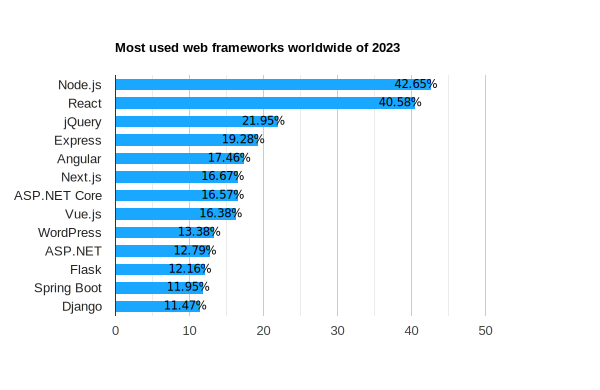
\includegraphics{diagrams/frameworkGraphs}
    \caption{Srovnání webových frameworků pro rok 2023 \cite{framework_comparison}}
    \label{fig:framework_comparison}
\end{figure}

\section{Zpracování požadavku}
\label{sec:dev-request-processing}
Zpracování požadavku patří do důležitých prvků webových aplikací. Vzhledem k~rozsáhlým rozdílům u~frameworků je nutné si blíže představit, jak takové zpracování probíhá. V~rámci tohoto procesu se setkáváme se dvěma typy zpracování -- \textit{Server-Side} a~\textit{Client-Side}. Jako třetí druh zpracování se dá považovat i~\textit{Hybridní} neboli \textit{Pre-Rendering}, který kombinuje oba přístupy.

Při vývoji je nutné si předem určit, který ze stylů zpracování bude pro projekt použit, přechod mezi jednotlivými druhy již v~průběhu vývoje může být velmi zdlouhavý a~finančně náročný. \cite{request_processing}

\subsection{Server-Side Rendering}
\label{subsec:dev-request-processing-server-side-rendering}
Server-Side Rendering (SSR) je často využívaný způsob zpracování, který se obvykle uplatňuje u~menších webových aplikací, které bývají označovány jako statické stránky, jež svůj obsah po zpracování již nikdy nemění. Základem SSR je, že veškeré zpracování dat probíhá na straně serveru, a~klient poté již obdrží kompletně vykreslenou stránku, kterou prohlížeč jednoduše načte. Tyto stránky díky své statické povaze dosahují vysokých hodnocení v~SEO, což je klíčové pro zvýšení návštěvnosti.

Jednou z~nevýhod SSR je však vysoká náročnost na výpočetní výkon serveru. Tento problém se projevuje zejména v~případě, kdy server zaznamená velké množství klientských požadavků v~krátkém časovém období. Při každém požadavku dojde k~novému kompletnímu vykreslení stránky, i~když se obsah stránky změnil jen minimálně.

\begin{figure}[H]
    \centering
    \includegraphics[width=1.0\textwidth]{figures/server-side-rendering}
    \caption{Postup Server-Side renderingu při žádosti o~stránku \cite{rendering-diff}}
    \label{fig:server-side-rendering}
\end{figure}

\subsection{Client-Side Rendering}
\label{subsec:dev-request-processing-client-side-rendering}
Client-Side Rendering (CSR) je moderní způsob zpracování webových stránek, jehož využití se rozšířilo s~příchodem programovacího jazyka JavaScript do světa World-Wide-Web (WWW). Tento přístup umožňuje dynamické vykreslování obsahu stránek přímo na straně klienta, což výrazně snižuje zátěž serveru a~zvyšuje rychlost zpracování požadavků.

Ve srovnání s~Server-Side Renderingem (SSR) je u~CSR náročnější dosáhnout vysokého skóre v~oblasti SEO. Důvodem je, že proces vykreslování stránky u~klienta může trvat proměnlivě dlouho a~existují rizika, že webcrawler, který indexuje stránku, ji opustí ještě před jejím kompletním načtením. Tento problém lze řešit pomocí techniky \textit{Pre-Rendering}, kterou popisuji v~následující sekci.

\begin{figure}[H]
    \centering
    \includegraphics[width=1.0\textwidth]{figures/client-side-rendering}
    \caption{Postup Client-Side renderingu při žádosti o~stránku \cite{rendering-diff}}
    \label{fig:client-side-rendering}
\end{figure}

\subsection{Hybrid Rendering}
\label{subsec:dev-request-processing-hybrid-rendering}
Hybrid Rendering, také známý jako Pre-Rendering, představuje moderní přístup k~zpracování webových stránek, který se pokouší o~skloubení výhod Server-Side a~Client-Side renderingu. Tento přístup jednoduše umožňuje vývojářům vytvářet takzvané \textquote{skeleton} stránky, které jsou odeslány klientovi ihned po přijetí požadavku. Po následném načtení stránky klientem, dochází k~dynamickému vykreslení obsahu, kde dojde k~nahrazení pouze daných části webu, které obsahovaly dynamický obsah.

\section{Technologie}
\label{sec:dev-technology}
V~této sekci se zaměřím na bližší popis technologií, které lze využívat během vývoje nebo přímo v~rámci daného frameworku. Mezi tyto technologie spadá široké spektrum nástrojů, knihoven, jazyků a~dalších prvků, které jsou volně dostupné na internetu a~mají za cíl usnadnit vývoj a~zvýšit efektivitu vývojáře.

\subsection{Šablonování}
\label{subsec:dev-technology-templating}
Šablonování je klíčovou technologií v~rámci vývoje webových aplikací, která slouží k~oddělení prezentace dat od logiky jejich zpracování. Tento přístup umožňuje vývojářům a~designérům efektivně spolupracovat na vytváření jak statických, tak dynamických uživatelských rozhraní, zatímco zvyšuje modularitu, udržitelnost a~bezpečnost kódu. Šablonování se většinou využívalo jako externí knihovna, ale s~příchodem moderních frameworků jako je Django, React nebo Angular se stalo nedílnou součástí těchto frameworků.

Jako systém umožňuje definovat strukturu a~vzhled webových stránek pomocí šablon, které se na sebe mohou vázat nebo se rozšiřovat. Každá z~těchto šablon obsahuje statický HTML kód spolu s~vloženými proměnnými, filtry a~řídícími strukturami. Finální šablony se poté před odesláním klientovi zpracují na serveru, a~je mu odeslám přímo výsledný HTML kód.

\noindent
Mezi hlavní výhody používání šablon patří:
\begin{enumerate}
    \item \textbf{Oddělení prezentace a~logiky:} Šablonovací systém oddělením prezentace dat a~logiky zpracování umožňuje vývojářům a~designérům efektivně spolupracovat.
    \item \textbf{Univerzální použitelnost:} Šablony lze použít pro vytváření jak statických, tak dynamických uživatelských rozhraní, což zvyšuje modularitu a~znovupoužitelnost kódu.
    \item \textbf{Podpora dynamických dat:} Díky použití proměnných a~filtrů umožňuje šablonovací systém dynamicky zobrazovat data na stránkách. To je klíčové pro vytváření interaktivních a~daty řízených uživatelských rozhraní.
    \item \textbf{Zabezpečení:} Systém frameworku obsahuje mechanismy pro prevenci útoků jako Cross-Site Scripting (XSS), Form tampering, SQL injection a~další. Tato zabezpečení jsou automaticky aplikována na šablony, což zvyšuje bezpečnost aplikace.
\end{enumerate}

Celkově lze konstatovat, že technologie šablonování přispívá k~efektivnímu a~strukturovanému vývoji webových aplikací, usnadňuje spolupráci mezi vývojáři a~designéry a~zvyšuje obecnou robustnost aplikace. Pro svůj projekt jsem zvolil šablonovací systém \textbf{Django Template Language (DTL)}, který je součástí frameworku Django.

\lstinputlisting[language=HTML, caption={Příklad použití templatu v~Djangu}, label={lst:django-template-example}]{sourceCodes/DjangoTemplateExample.html}

Na výše uvedeném zdrojovém kódu lze vidět několik \textit{block} značek, které rozdělují šablonu na jednotlivé části. Tyto bloky lze později implementovat v~jiných šablonách, kde se daná šablona rozšiřuje. Na řádku 19. můžeme vidět, že sekce \textit{content} bude později implementována.

\subsection{Boostrap}
\label{subsec:dev-technology-bootstrap}
Bootstrap je open-source framework, který byl původně vytvořen firmou Twitter s~hlavním cílem zjednodušit vývoj konzistentních a~responzivních uživatelských rozhraní pro webové aplikace a~stránky. Tento framework se stal díky jeho modularitě a~flexibilitě jedním z~nejpopulárnějších nástrojů pro vývojáře a~designéry.

Jeho klíčovou vlastností, která přímo navazuje na principy responzivního designu~\ref{subsec:ui-gui-theory-responsive-design} zmíněné v~předchozí podkapitole, je použití tzv. \textit{Grid systému}, tedy rozložení mřížky. Tento systém Boostrapu umožňuje vývojářům snadno vytvářet komplexní rozložení stránek za použití základních předdefinovaných tříd, které určují šířku sloupců, vnitřní a~vnější okraje a~další. Při změně velikosti obrazovky pak dojde v~systému k~automatickému přizpůsobení velikosti jednotlivých oken, čímž nevzniknou žádné problémy s~rozložením komponent.

Bootstrap neobsahuje pouze předdefinovaný CSS třídy, ale i~nemalé množství JavaScriptových pluginů, které rozšiřují funkčnost základních komponent HTML o~interaktivitu. Příkladem takové komponenty může být například \textit{Dropdown}, \textit{Modal}, \textit{Carousel} a~další.

V~praxi lze tento systém velmi snadno implementovat do jakéhokoliv projektu. Pro jeho implementaci stačí přidat odkazy na soubory CSS a~JavaScript do hlavního HTML dokumentu, po správném vložení lze ihned začít využívat komponent Bootstrapu. Díky této praktiky je možné urychlit vývoj prototypů, aniž by bylo nutné psát vlastní styly.

\endinput
\chapter{Implementace}
\label{ch:implementation}

\section{Požadavky na implementaci}
\label{sec:implementation-requirements}

\section{Komponenty aplikace}
\label{sec:implementation-components}

\subsection{Frontend}
\label{subsec:implementation-frontend}

\subsection{Backend}
\label{subsec:implementation-backend}

\subsection{API}
\label{subsec:implementation-api}
Práce s API přes middleware, který zabezpečuje správné použití klíče.

\section{Volba technologií}
\label{sec:implementation-technologies}

\subsection{Framework}
\label{subsec:implementation-technologies-framework}
Zvoleno Django, odkaz na analýzu frameworku.

\subsection{Database}
\label{subsec:implementation-technologies-database}
Zvolena MariaDB. Výhody nevýhody porovnání ostatních. PostgreSQL, ...

\subsubsection*{Schéma}
\label{subsubsec:implementation-technologies-database-scheme}
Diagram schéma databáze -> Diagram

\subsubsection*{Automatizace}
\label{subsubsec:implementation-technologies-database-automatization}
Popis tvorby skriptu pro naplnění databáze. Priorita plnění. -> Diagram

\section{Týmová spolupráce}
\label{sec:implementation-collaboration}
Týmová spolupráce ve čtyřčlenném týmu studentů se stává obzvláště komplikovaná v době, kdy je projekt rozdělen do separátních části, které jsou na sebe závislé a je tak nutná vzájemná komunikace a spolupráce. Jako hlavní komponentou této práce se tak stává API, která slouží pro kompletní komunikaci v rámci projektu. V této sekci se tak zaměřím na to, jak jsme si rozdělili práci, jak jsem postupovali a následně řešili problémy, které vznikaly.

\subsection{Rozdělení práce}
\label{subsec:implementation-collaboration-distribution}
Rozdělení práce v týmu bylo provedeno tak, že každý člen měl dle zadání přidělenou určitou hlavní část projektu, za kterou byl plně zodpovědný. Každá z těchto částí projektu pak byla následně rozdělena na menší sekce, na kterých se daní členové podíleli buď samostatně nebo ve spolupráci. Spolupráce je tak zobrazena v šedém boxu, kde její vnitřní barevné čtverec reprezentuje daného člena. Ve výsledném rozdělení práce na obrázku~\ref{fig:job_distribution} také lze také jednoduše rozlišit obtížností nebo velikostní rozdíl pod částí.

\begin{figure}[h]
    \centering
    \includegraphics[width=0.95\textwidth]{../../shared/diagrams/blocks}
    \caption{Rozložení práce v týmu}
    \label{fig:job_distribution}
\end{figure}

\subsection{Verzování kódu}
\label{subsec:implementation-collaboration-versioning}
Efektivnost verzování kódu je důležitou součástí každé týmové spolupráce na větším projektu. Pro správu obsahu práce jsem tak využili nástroj Git pod službou GitHub, který nám umožnil efektivně sledovat změny a udržovat si tak přehled o vývoji projektu. Využití Gitu bylo zvoleno především pro jeho jednoduchost a znalost všech členů týmu, kteří s ním již měli zkušenosti v minulosti.

%Pro zajištění správného vývoje byly vytvořeny dvě hlavní větve, které sloužily pro vývoj nových funkcí a opravu chyb. Větve byly následně spojovány pomocí pull requestů, které sloužily pro kontrolu a schválení změn. Tento proces byl zvolen pro zajištění kvality kódu a zamezení chybám, které by mohly vzniknout při nesprávném spojení větví.

\subsubsection*{Větve}
\label{subsubsec:implementation-collaboration-versioning-branches}
V moderních vývojích systému se každá část nebo project celý rozděluje do složitějšího stromu větví známého pod názvem \textit{Git Worfkflow}, jeho efektivní reprezentaci lze vidět na obrázku~\ref{fig:git_workflow}. Tento strom se dělí na 2 hlavní větve, často nazývané \textit{master} a \textit{develop}.

Větev \textit{master} slouží pro produkční verze projektu, které jsou připraveny k nasazení, zatímco větev \textit{develop} slouží pro vývoj nových funkcí. Aktualizace větví tzv. \textit{commits} jsou poté spojovány pomocí pull requestů, které slouží pro kontrolu a schválení změn. Tento proces byl zvolen pro zajištění kvality kódu a zamezení chybám, které by mohly vzniknout při nesprávném spojení větví.

Následně strom obsahuje pod větve vývojové, tyto větve se často štěpí z větve developu a slouží pro vývoj nových funkcí nebo opravu chyb. Po dokončení a úspěšném testování je tato větev spojena zpět do developu a po vydání nové verze je spojena do masteru.

\subsubsection*{Zkratky}
Tabulka zkratek zobrazena v obrázku ~\ref{fig:git_workflow}.

\begin{table}[h]
    \centering
    \resizebox{\textwidth}{!}{%
        \begin{tabular}{l l l}
            \toprule

            \textbf{Příkaz} & \textbf{Zkratka} & \textbf{Význam} \\
            \midrule

            \textbf{git nh} & New Hotfix & Vytvoření větve pro rychlou opravu chyb, která je již v produkci \\
            \textbf{git mh} & Merge Hotfix & Dokončení vývoje a spojení větve zpět do masteru \\
            \textbf{git live} & Release & Publikace nové verze a spojení větve do masteru \\
            \textbf{git nb} & New Bugfix & Vytvoření větve pro opravu chyb, která je ve vývoji \\
            \textbf{git mb} & Merge Bugfix & Dokončení vývoje a spojení větve zpět do developu \\
            \textbf{git uat} & User Acceptance Testing & Vytvoření větve pro testování nové verze \\
            \textbf{git nf} & New Feature & Vytvoření větve pro vývoj nové funkce \\
            \textbf{git mf} & Merge Feature & Dokončení vývoje a spojení větve zpět do developu \\

            \bottomrule
        \end{tabular}}
    \caption{Seznam efektů}
    \label{tab:effects}
\end{table}

%Informace o verzování kódu. Jak se používá Git, jak se vytvářejí větve, jak se dělají pull requesty, jak se řeší konflikty.
%https://www.freecodecamp.org/news/how-to-use-git-best-practices-for-beginners/
%https://stackoverflow.com/questions/19695127/git-workflow-review

\begin{figure}[H]
    \centering
    \includegraphics[width=0.9\textwidth]{figures/GitWorkflow}
    \caption{Ukázka správného použití verzovacího systému Git. \cite{git_workflow}}
    \label{fig:git_workflow}
\end{figure}

\subsection{Sdílení kódu}
\label{subsec:implementation-collaboration-sharing}

\section{Problémy vývoje}
\label{sec:implementation-problems}

\subsection*{Hexagonální grid}
\label{subsec:implementation-problems-hexagon}

%\newpage
%\processDiagram{diagrams/OpenPage}{OpenPage}{0.75\textwidth}{Diagram aaa}
%
%\newpage
%\processDiagram{diagrams/NewObject}{NewObject}{0.75\textwidth}{Diagram průběhu editace nebo přidávání dat}

\endinput

% Zaver
\chapter{Závěr}
Tato bakalářská práce se zaměřila na tvorbu uživatelského prostředí pro výpravnou evoluční hru, která kombinuje prvky stolní a počítačové hry. Cílem práce bylo vytvořit funkční prototyp uživatelského prostředí, který bude schopen zobrazit herní svět a umožní hráčům provádět herní akce. Práce byla rozdělena do několika částí, které se postupně zabývaly historií hybridních stolních her, problematikou vývoje grafických rozhraní a návrhem a implementací grafického rozhraní pro výpravnou evoluční hru.

V úvodu práce byla popsána historie hybridních stolních her a jejich vývoj od propojování jednoduchých elektrických obvodů až po moderní hry, které mívají vlastní aplikace, či celé elektronické zařízení. Následně byla pojednána problematika a zásady vývoje grafických rozhraní a tyto zkušenosti byly předvedeny na pomocných aplikacích pro stolní hry \textit{Na vlnách neznáma} a \textit{Gloomhaven}.

Práce se dále zabývala návrhem a implementací grafického rozhraní pro výpravnou evoluční hru. V rámci tohoto návrhu byly srovnány použitelné technologie pro tvorbu grafických rozhraní a byly vybrány ty, které byly považovány za nejvhodnější. Dále byly navrženy fyzické herní komponenty a herní mechaniky, které byly následně implementovány v prototypu uživatelského prostředí. Výsledkem práce je funkční prototyp uživatelského prostředí, který je schopen zobrazit herní svět a umožňuje hráčům provádět herní akce. Tento prototyp byl následně otestován několika jednotlivci, kteří poskytli cenné zpětné vazby, které byly použity k vylepšení prototypu uživatelského prostředí.

Výsledek práce byl propojen s pracemi ostatních spoluřešitelů, což vedlo k vytvoření funkčního prototypu celé stolní hry. Tento prototyp byl následně otestován odehráním několika herních situací. Z těchto testů vyplynulo, že prototyp je správně schopen plnit funkce, k nímž byl navržen.

% Prilohy
\appendix
\chapter{Database Scripts Output}
\label{ch:appendix-database-scripts-output}

\begin{figure}[h]
    \centering
    \includegraphics[width=1.0\textwidth]{figures/dbScriptsOutput}
    \caption{Výstup skriptů pro vytvoření databáze.}
    \label{fig:databaseScriptsOutput}
\end{figure}

\endinput

% Seznam literatury
\printbibliography[title={Literatura}, heading=bibintoc]

\end{document}
